\documentclass[letter,11pt,oneside,spanish]{article}

\usepackage[utf8x]{inputenc}
\usepackage[spanish]{babel}
\usepackage{graphicx}
\usepackage{float}
\usepackage{anysize}

\usepackage[
pdfauthor={Carlos Caballero},%
pdftitle={Babel},%
colorlinks,%
citecolor=black,%
filecolor=black,%
linkcolor=black,%
%urlcolor=black
pdftex]{hyperref}

\marginsize{2.5cm}{2.5cm}{2.5cm}{2.5cm}
\renewcommand{\baselinestretch}{1.5}

%opening
\title{\textbf{Babel: Servidor de libros digitales}}
\author{Carlos Caballero\\
Documento de Investigación\\
Universidad Mayor de San Simón\\
\{cijkb.j@gmail.com\\}
\date{}
\begin{document}

\begin{titlepage}
\thispagestyle{empty}
\begin{center}
\large{\textsc{\bf Universidad Mayor De San Simón}}\\
\large{\textsc{\bf Facultad De Ciencias y Tecnología}}\\
\large{\textsc{\bf Sociedad Científica de Informática y Sistemas}}\\
\vspace{4.0cm}
\large{\bf Reducción de las brechas de acceso a la información\\
a partir del intercambio libre de recursos de aprendizaje}\\
\vspace{1.0cm}
\small{Carlos Eduardo Caballero Burgoa}
~\\
\small{\today}
\end{center}
\end{titlepage}

\newpage
\tableofcontents

\newpage
\section{Introducción}
El propósito de este documento es resumir todo el proceso de investigación
llevado a cabo para la construcción de una solución factible al problema del
intercambio de información entre personas. A partir del desarrollo de un sistema
web al me referiré como: 'Babel'.

Babel es una de las piezas de software desarrolladas en la sociedad científica
de sistemas e informática (UMSS); que esta encaminada a reducir las brechas de
acceso a la información que se ha percibido entre la comunidad estudiantil.
Esencialmente consiste en un sitio web desarrollado en el lenguaje de
programación PHP, donde los usuarios pueden compartir, ordenar, clasificar, y
catalogar archivos en formato PDF.

Esta solución ha sido concebida con un lógica descentralizada de intercambio, es
decir, esta diseñada para crear multiples conexiones con otras instancias, ya
sean publicas o privadas, de modo que el rango de búsqueda pueda propagarse a
una variedad aún mayor que la de una única instancia (P2P).

\section{Antecedentes}
Debido a que no contamos con una biblioteca virtual en los predios de la
universidad, surgió la idea de realizar un proyecto que trate de crear un centro
de información electrónico que proporcione documentos a sus usuarios.

Si bien los problemas de accesibilidad a los recursos de información se han
visto reducidos por el cada vez mayor acceso a Internet, aún el problema esta
vigente, dadas esas condiciones se intentó subsanar algunos aspectos de esta.
Después de mucho analizar la situación, se concluyó que el conjunto de
dificultades que tienen las personas, pueden ser clasificadas en cuatro tipos:

\begin{description}
\item [Problemas de acceso a la información]
    Referentes a los problemas de acceso al recurso necesario.
\item [Problemas de falta de conocimiento]
    Referentes al desconocimiento acerca del área sobre el que una persona esta
    inmerso.
\item [Problemas de disponibilidad de tiempo]
    Referentes a los problemas en los que el tiempo requerido para alcanzar
    el objetivo no puede ser cubierto.
\item [Problemas de compromiso]
    Referentes a los problemas en los que la intención por hacer lo requerido es
    la carencia principal de las personas.
\end{description}

Entendiendo este conjunto de problemas, se ha definido como objetivo del
proyecto babel: Minimizar los problemas de acceso a la información, siendo esta
la primera barrera que se tiene al intentar alcanzar los objetivos deseados.

\section{Justificación}
Ya no sera necesario desplazarse hasta una biblioteca o un centro de
documentación para conseguir la información que necesitemos, se podrá acceder a
la información almacenada en soporte digital (a distancia) y obtenerla al
momento.

Pero más allá del acceso a Internet, la existencia de la brecha digital es la
demostración de una nueva barrera al acceso al conocimiento y al desarrollo
económico para los países pobres \cite{brecha}. Por ende viabilizar el
intercambio y colaboración entre las personas, es un paso determinante para el
avance tecnologico en general.

\section{Planteamiento del Problema}
En la Universidad de San Simón, normalmente el acceso a Internet es para unos
pocos afortunados; el resto de la población estudiantil solo posee acceso a un
conjunto muy pobre de paginas de información interna. Considerando las estrictas
políticas que posee esta universidad para sus tecnologías de información y
comunicación, se hizó notoria la falta de un espacio comun de intercambio que
este orientado a los estudiantes.

Ademas se ha notado que si bien las personas quieren compartir sus recursos, los
canales de comunicación para hacerlo son difíciles, y escasos, lo cual conlleva
a crear metodos en extremo ineficientes para el intercambio, ademas de ser gran
desperdicio de recursos y tiempo para toda la comunidad.

\section{Formulación del Problema}
Considerando los antecedentes mencionados anteriormente, se puede concluir que:

\begin{itemize}
\item Existen reducidas opciones para el intercambio de información entre
estudiantes.
\item Todas las soluciones actuales son ejecutadas en un modo descentralizado y
manual.
\item Se reducen las aptitudes de los estudiantes con respecto a compartir e
intercambiar el conocimiento que estos poseen.
\end{itemize}

Por lo mencionado anteriormente se define el problema como:

\emph{La amplia variedad de información, y su carencia de organización;
dificulta a los estudiantes adquirir el conocimiento que ellos pretenden
alcanzar.}

\section{Objetivo General}
Minimizar los problemas de acceso a la información para facilitar la adquisición
de conocimiento para mejorar los metodos de adquisición de conocimiento.

\section{Objetivos Específicos}
\begin{itemize}
\item Facilitar la clasificación e intercambio de recursos para simplificar los
procesos cotidianos inherentes en estas tareas.
\item Ampliar los canales de intercambio de recursos entre las personas para
mejorar la disponibilidad de estos entre los usuarios.
\item Agilizar los procesos de publicación, y clasificación de recursos para
simplificar muchas de las tareas necesarias de administración.
\end{itemize}

\section{Hipótesis}
Con este proyecto intento demostrar que brindando un conjunto de servicios que
faciliten los métodos de intercambio de información (es decir, reducir la brecha
de acceso a la información), se pueden agilizar y posibilitar grandes
posibilidades para la mejora de los metodos de adquisición de conocimiento en la
población estudiantil.

\section{Aporte científico}
Se ha desarrollado el sistema bajo una arquitecura orientada a servicios, que
se ejecuta como un sistema web escrito en el lenguaje de programación PHP, y ha
sido probado sobre servidores Apache Web Server y Nginx; se tomo esta decisión
basados en las estadisticas de uso de este lenguaje y estos servidores, haciendo
del sistema una herramienta facíl de desplegar.

Se ha investigado mucho en estructuras de datos (ademas de sistemas de
clasificación, y biblioteconomía), para facilitar el manejo de catálogos (ver
siguiente sección), ademas de desarrollar muchas utilidades para automatización
en las tareas de publicación, categorización, y clasificación de recursos.

\section{Diseño metodológico y teórico}
Se ha estructurado el proyecto en cuatro grandes tareas:

\begin{description}
\item [Busqueda de documentos]
    Se diseño una ontologia de busqueda para los documentos, y se utilizó el
    motor de busqueda Lucene para la implementación de las funciones de busqueda
    de documentos.
\item [Intercambio de documentos]
    Se ha construido una gran cantidad de utilidades para la automatización de
    tareas comunes, de modo que puedan ser compartidos grandes volumenes de
    información. Se utilizo el algoritmo SHA256, para crear identificadores
    únicos de los documentos compartidos.
\item [Clasificación de documentos]
    Al principio se consideraron varios metodos de catalogación, basados en los
    métodos utilizados en el area de biblioteconomía, se analizó el sistema de
    clasificación decimal de Dewey, el sistema de clasificación colonada, entre
    otros.
    En la actualidad el sistema ha sido diseñado para soportar multiples
    sistemas de clasificación de libros, ya sean estos taxonomicos y
    folcsonomicos.
\item [Valoración de documentos]
    Se utilizaron algunos conceptos de inteligencia colectiva y web 2.0 para
    poder facilitar la busqueda de posibles documentos utiles para un usuario
    basado en las apreciaciones subjetivas de otros usuarios del mismo sistema.
\end{description}

\section{Desarrollo del proyecto}
Despues de muchos años de desarrollo y refactorización de las funciones, se
obtuvo una versión estable del sistema. Este se encuentra alojado actualmente
en el sitio \url{http://babel.scesi.org}, y se ha publicado el codigo fuente del
mismo en el sitio \url{https://github.com/ccaballero/babel} para la instalación
libre de otras instancias descentralizadas.

\section{Conclusiones y recomendaciones}
Si bien el sistema esta en ejecución hace muchos meses, se ha notado muy poco
trafico hacia este, a pesar de la gran cantidad de información disponible en
este; haciendo de la mineria de datos, y la valoración de indicadores medibles
algo muy poco efectivo.

Se han planteado estrategias de difusión, para conseguir enriquecer el conjunto
de personas que utilizen el sistema, aún esta por verse donde termina.

\newpage
\begin{thebibliography}{99}
    \bibitem{brecha}
        \textsc{Arial Sar.:}
        \textit{\textbf{La Brecha del Conocimiento y la Brecha Digital.}}
        \par Mayo, 2004.
\end{thebibliography}

\newpage
\begin{figure}
 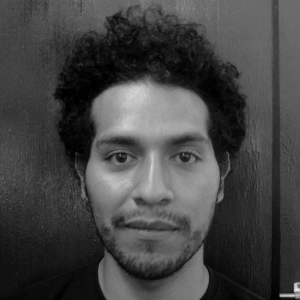
\includegraphics[scale=0.3]{jacobian.jpg}
\end{figure}
\textbf{Univ. Carlos Eduardo Caballero Burgoa}\\
Estudiante de Ing. de Sistemas en la Universidad Mayor de San Simón, Miembro de la sociedad cientifica
de Informática y Sistemas y Administrador del Laboratorio de Desarrollo del Departamento de
Informática y Sistemas.

\end{document}